\documentclass[11pt,a4paper]{article}
\usepackage{amsmath}
\usepackage{amsfonts}
\usepackage{amssymb}
\usepackage{makeidx}
\usepackage{graphicx}
\usepackage{wrapfig}
\usepackage{enumerate}
\usepackage{pdfpages}
\usepackage{tocloft}
\usepackage{setspace}
\usepackage{mathtools}
\usepackage{hyperref}
\definecolor{linkcolour}{rgb}{0,0.2,0.6} % Link color
\hypersetup{colorlinks,breaklinks,urlcolor=linkcolour,linkcolor=linkcolour}

\usepackage[left=2cm,right=2cm,top=2cm,bottom=2cm]{geometry}

\usepackage{xcolor}

%\usepackage{fontspec}
%\setmainfont{Cambria}

\usepackage{caption}
\captionsetup[figure]{font=small, labelfont={bf}}
\captionsetup[table]{font=small, labelfont={bf}}

\usepackage{float}
\usepackage{multirow}
\usepackage{longtable}

\usepackage[nottoc]{tocbibind}

\newcommand{\spa}{\vspace{1.25em}}
\newcommand{\noi}{\noindent}
\def\dul#1{\underline{\underline{#1}}}
\def\cpt#1#2{{\begin{center}\small\textbf{\textcolor{blue}{Figure #1:}} #2\end{center}}}
\def\tt#1{\texttt{#1}}

% for dots in the content
\usepackage{tocloft}
\renewcommand{\cftsecleader}{\cftdotfill{\cftdotsep}}

\begin{document}
	\begin{titlepage} 
		\begin{center}
		\large{ASSIGNMENT 2}\\
		\vspace{2em}
		\large {CS5691 Pattern Recognition and Machine Learning}
		\vspace{3em}
		
		\rule{0.9\linewidth}{0.5mm} \\[0.4cm]
	    {\Large{\bfseries{CS5691 Assignment 2}}} \\
	    \rule{0.9\linewidth}{0.5mm} \\[3 em]	
	    
	    Team Members: \\
	    \vspace{0.5em}
	   	\def\arraystretch{1.25}
\begin{tabular}{c l}
	\hline
	BE17B007 & N Sowmya Manojna \\
	PH17B010 & Thakkar Riya Anandbhai \\
	PH17B011 & Chaithanya Krishna Moorthy \\
	\hline
\end{tabular}

		\vspace{1em}

		Indian Institute of Technology, Madras\\    
		
		\vspace{5em}    
	    
	    	
\includegraphics[scale = 0.09]{images/iitmlogo.png}
		\end{center}
	\end{titlepage}

{\hypersetup{linkcolor=black}
 \tableofcontents}
\break


\section{Dataset 1A}
\subsection{K-nearest Neighbors Classifier}
\subsection{Naive-Bayes classifier}
\subsubsection{Same Covariance Matrix ($\sigma^2I$)}
\subsubsection{Same Covariance Matrix ($C$)}
\subsubsection{Different Covariance Matrix}

\break
\section{Dataset 1B}
\subsection{K-nearest Neighbors Classifier}
\subsection{Bayes Classifier, GMM, full covariance}
\subsubsection{Equations}
Th initialization is done as follows for each class:
\begin{itemize}
    \itemsep0em
    \item Cluster initialization is using \tt{kmeans} clustering.
    \item The relative number of points in each cluster $N_q$ and weightage $w_q$ for each cluster is calculated.
    \item The responsibility $\gamma_{n,q}$ is then calculated, followed by mean $\mu_q$ and covariance $C_q$ is calculated.
\end{itemize}

\noi
The parameters are then updated sequentially through the:
\begin{itemize}
    \itemsep0em
    \item Expectation-step: $\gamma_{n,q}$ is updated.
    \item Maximization-step: $\mu_q$, $C_q$, $N_q$ and $w_q$ are updated.
\end{itemize}

\noi
The stopping criterion used is $\Delta(\text{likelihood})<\tt{tol}$. The \tt{tol} we considered is $10^{-5}$.\\

\noi
Based on the accuracies obtained on the training, validation and test dataset, the best $q_i$ for the three classes has been chosen as $5$.
\subsubsection{Training and Validation Accuracy}
The training and validation accuracies obtained for varying $q_i$ for each class is as follows:
\begin{figure}[H]
    \hspace{-2em}
    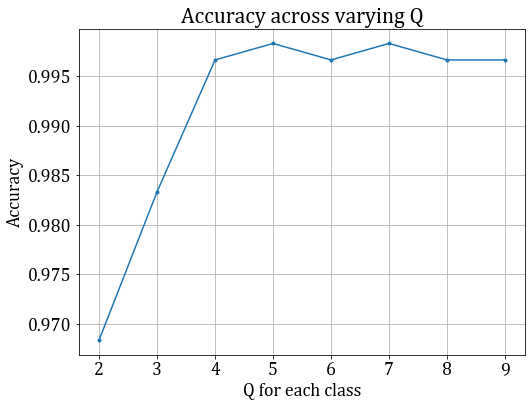
\includegraphics[scale=0.5]{images/1b_full_train.png}
    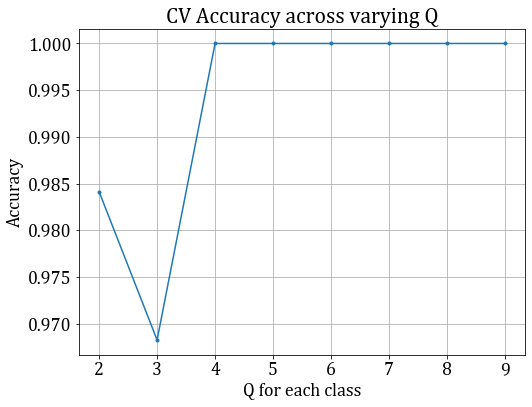
\includegraphics[scale=0.5]{images/1b_full_val.png}
    \caption{Training and Validation accuracy across $q_i$, on the left and right respectively}
\end{figure}

\subsubsection{Testing Accuracy}
The testing accuracy obtained for varying $q_i$ for each class is as follows:
\begin{figure}[H]
    \centering
    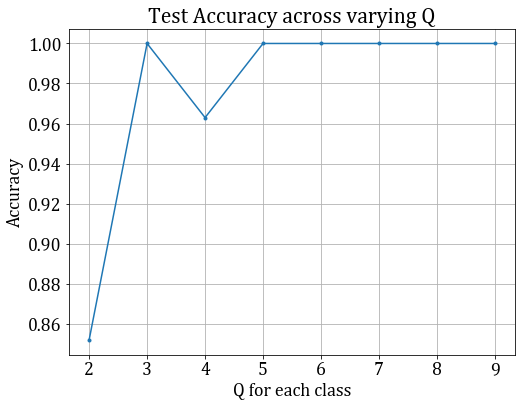
\includegraphics[scale=0.5]{images/1b_full_test.png}
    \caption{Testing accuracy across $q_i$}
\end{figure}

\subsubsection{Contour Maps and Decision Surfaces}
The contour maps and decision surfaces obtained, with $q_i=5$ are as follows:
\begin{figure}[H]
    \hspace{-1em}
    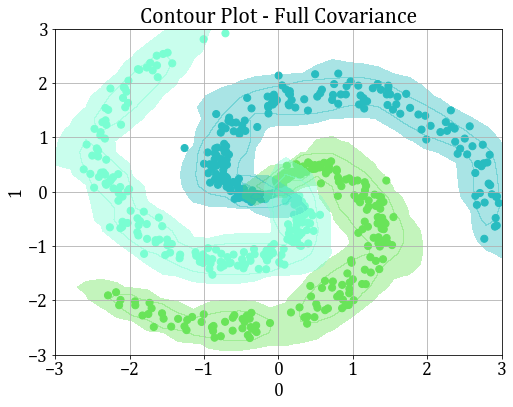
\includegraphics[scale=0.5]{images/1b_full_contours.png}
    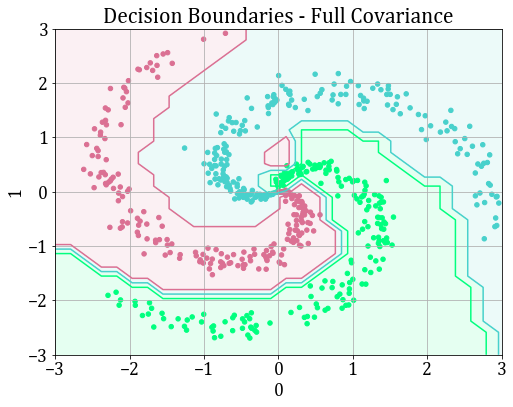
\includegraphics[scale=0.5]{images/1b_full_decision_surfaces.png}
    \caption{Contour Maps and Decision Surfaces obtained for $q_i=5$, on the left and right respectively}
\end{figure}


\subsection{Bayes Classifier, GMM, diagonal covariance}
\subsubsection{Training and Validation accuracy}
Gaussian multi-modal training function (with threshold of the increment in total log-likelihood functions as 0.01 since there was no significant improvement for a smaller threshold than this) with diagonal covariance matrix over the hyperparameter values of the number of gaussian components Q = {2,3,4,5,6,7,8,9} to estimate the parameters - $\mu_q$, $C_q$, $N_q$ and $w_q$ for each gaussian component - and predict the classes of the training data (train.csv) and cross-validation (70\% of dev.csv), we get the table \ref{tab:cv1b}
\begin{table}[H]
\centering
\begin{tabular}{l l l }
\hline
\hline
\textbf{Hyperparameter Value (Q)} &  \textbf{Accuracy on CV data} &  \textbf{Accuracy on Training data}  \\
\hline
\hline
2 & 0.873 & 0.9166\\
3 & 0.920 & 0.976\\
4 & 0.968 & 0.9966\\
5 & 0.984 & 1.0\\
6 & 0.984 & 0.986\\
7 & 0.984 & 0.991\\
8 & 0.984 & 0.9916\\
9 & 0.984 & 0.9916\\
\hline
\end{tabular}
\caption{Variation of Accuracy across Hyperparameter values on the validation data using the GMM model with diagonal covariance matrix on Dataset 1B}
\label{tab:cv1b}
\end{table}


\begin{figure}
    \centering
    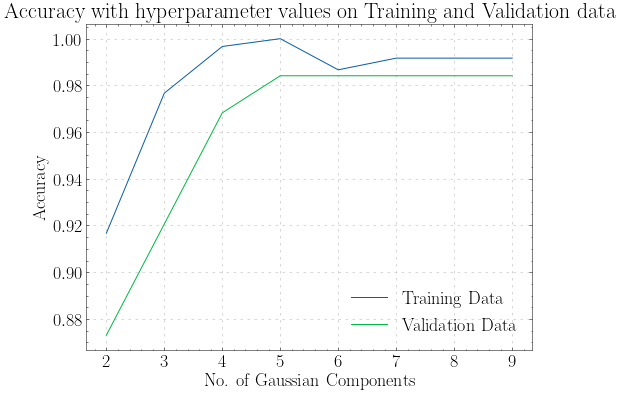
\includegraphics[scale=0.5]{images/acc_1b.png}
    \caption{Plot of Hyperparameter value Vs Accuracy using the GMM model with diagonal covariance matrix on Dataset 1B}
    \label{fig:acc1bGMMdiag}
\end{figure}
\subsubsection{Best model output}
As we can see in the tables and figure \ref{fig:acc1bGMM}, the best accuracy is when the number of Gaussian components is 5. Using the parameters of the model for 5 gaussian components and predicting for the test dataset (30\% of dev.csv), the accuracy obtained was \textbf{1.0}.\\
The confusion matrices for the training and test datasets using the best model are tables \ref{tab:conf_train1b} and \ref{tab:conf_test1b}.\\
\begin{table}[H]
\centering
\begin{tabular}{|l|l|l|l|}
\hline
&0&1&2\\
\hline
0&200&0&0\\
\hline
1&0&200&0\\
\hline
2&0&0&200\\
\hline
\end{tabular}
\caption{Confusion Matrix for training data 1B}
\label{tab:conf_train1b}
\end{table}


\begin{table}[]
    \centering
    
        \begin{tabular}{|l|l|l|l|}
            \hline
            &0&1&2\\
            \hline
            0&9&0&0\\
            \hline
            1&0&10&0\\
            \hline
            2&0&0&8\\
            \hline
 \end{tabular}

\caption{Confusion Matrix for test data 1B}
    \label{tab:conf_train1b}
\end{table}

The decision region plot for the best model is figure \ref{fig:dec1bGMMdiag}
\begin{figure}
    \centering
    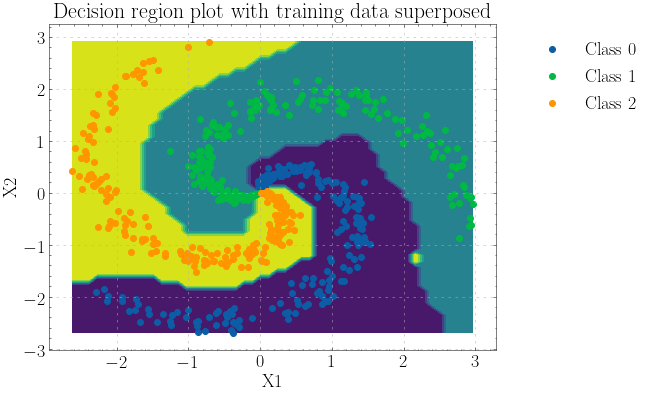
\includegraphics[scale = 0.5]{images/decisionReg_ds2.png}
    \caption{Decision region plot for Bayesian GMM model using diagonal covariance matrix and 5 gaussian components on dataset 1B}
    \label{fig:dec1bGMMdiag}
\end{figure}
\subsection{Bayes Classifier, KNN}

\break
\section{Dataset 2A}
\subsection{Bayes Classifier, GMM, full covariance}
\subsection{Bayes Classifier, GMM, diagonal covariance}
\subsubsection{Training and Validation Accuracy}
The accuracy obtained on training the data 2A on GMM model with diagonal covariance matrix is as in table \ref{tab:acc2a}. The plot of the same is in figure \ref{fig:acc2adiag}. The tolerence used was 1e-3.
\begin{table}[H]
\centering
\begin{tabular}{l l l l}
\hline
\hline
\textbf{# Clusters/Class (Q)} & \textbf{Training Accuracy} & \textbf{Validation Accuracy}\\
\hline
\hline
2 & 0.509 & 0.350\\
3 & 0.525 & 0.404\\
4 & 0.574 & 0.436\\
5 & 0.627 & 0.420\\
6 & 0.6491 & 0.418\\
\hl{7} & \hl{0.663} & \hl{0.440}\\
8 & 0.689 & 0.371\\
9 & 0.692 & 0.413\\
10 & 0.718 & 0.427\\
11 & 0.735 & 0.396\\
12 & 0.754 & 0.393\\
13 & 0.770 & 0.434\\
14 & 0.783 & 0.388\\
\hline
\end{tabular}
\caption{Variation of accuracy across hyperparameter values on the training and validation using the GMM model with diagonal covariance matrix on Dataset 2A. }
\label{tab:acc2a}
\end{table}


\begin{figure}
    \centering
    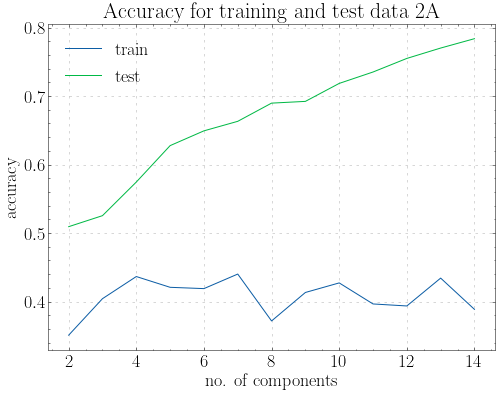
\includegraphics[scale = 0.5]{acc_2a.png}
    \caption{accuracy for training and validation set for 2A}
    \label{fig:acc2adiag}
\end{figure}
\subsection{Best model on test data}
The highest accuracy on validation data set is for 7 gaussian components. Applying this model to predict the test data, we get an accuracy of \textbf{0.37}. The confusion matrices for this model on training and test data are tables \ref{tab:conf_train2a} and \ref{tab:conf_test2a}.
\begin{table}[H]
\centering
\begin{tabular}{|l|l|l|l|l|l|}
\hline
 & 0 & 1 & 2 & 3 & 4 \\
\hline
0 & 147 & 8 & 21 & 22 & 35 \\
\hline
1 & 7 & 156 & 7 & 13 & 14 \\
\hline
2 & 39 & 5 & 165 & 30 & 45 \\
\hline
3 & 25 & 7 & 20 & 190 & 24 \\
\hline
4 & 33 & 6 & 36 & 32 & 143 \\
\hline
\end{tabular}
\caption{Confusion Matrix for training data 2A}
\label{tab:conf_train2a}
\end{table}

\begin{table}[]
    \centering
\begin{tabular}{|l|l|l|l|l|l|}
\hline
&0&1&2&3&4\\
\hline
0&37&4&11&12&7\\
\hline
1&5&25&6&3&4\\
\hline
2&12&10&27&19&20\\
\hline
3&9&8&12&40&21\\
\hline
4&10&5&15&8&23\\
\hline
\end{tabular}
\caption{Confusion Matrix for test data 2A}
    \label{tab:conf_train2a}
\end{table}


\break
\section{Dataset 2B}
\subsection{Bayes Classifier, GMM, full covariance}
\subsection{Bayes Classifier, GMM, diagonal covariance}


\end{document}